% ============================================================
%  IEEE Paper: FEC for 5G URLLC
%  Compile with: pdflatex → bibtex → pdflatex → pdflatex
%  Required packages: IEEEtran, amsmath, graphicx, tikz,
%                     pgfplots, booktabs, hyperref, algorithm2e
% ============================================================
\documentclass[conference]{IEEEtran}

\usepackage{amsmath,amssymb}
\usepackage{graphicx}
\usepackage{tikz}
\usepackage{pgfplots}
\pgfplotsset{compat=1.18}
\usepackage{booktabs}
\usepackage{multirow}
\usepackage{array}
\usepackage[ruled,vlined]{algorithm2e}
\usepackage[hidelinks]{hyperref}
\usepackage{cite}
\usepackage{xcolor}

\usetikzlibrary{shapes.geometric, arrows.meta, positioning, fit, backgrounds}

% TikZ style definitions
\tikzset{
  block/.style={rectangle, draw, text width=5em, text centered,
                rounded corners, minimum height=2.5em, fill=blue!10},
  wideblock/.style={rectangle, draw, text width=7em, text centered,
                    rounded corners, minimum height=2.5em, fill=green!10},
  decision/.style={diamond, draw, text width=4em, text centered,
                   fill=orange!15, inner sep=0pt},
  arrow/.style={->, >=Stealth, thick},
  lostpkt/.style={rectangle, draw, dashed, fill=red!15,
                  text centered, text width=4em, minimum height=2em},
  goodpkt/.style={rectangle, draw, fill=green!20,
                  text centered, text width=4em, minimum height=2em},
}

% ── Title / Authors ─────────────────────────────────────────────
\title{Forward Error Correction for Ultra-Reliable\\
       Low-Latency Communication in 5G Networks:\\
       A GF(256) Erasure Coding Approach}

\author{
  \IEEEauthorblockN{[Author Name]}
  \IEEEauthorblockA{Department of [Your Department]\\
    [Your Institution]\\
    Email: [your@email.edu]}
}

\begin{document}
\maketitle

% ============================================================
% I.  ABSTRACT
% ============================================================
\begin{abstract}
Fifth-generation (5G) wireless networks introduce the Ultra-Reliable
Low-Latency Communication (URLLC) service class, demanding packet
delivery reliabilities of 99.999\% with end-to-end latencies below
1\,ms. These requirements are fundamentally incompatible with
conventional retransmission-based error recovery, which introduces
intolerable uncontrollable delays in time-sensitive applications such as
autonomous vehicles, remote surgery, and industrial automation. The
heterogeneous 5G radio channel further exacerbates packet loss through
both independent (Bernoulli) fading events and correlated burst losses
modelled by the Gilbert--Elliott Markov chain.

Existing error-recovery mechanisms---including TCP retransmission, Hybrid
Automatic Repeat reQuest (HARQ), and prior FEC deployments based on
Reed--Solomon codes---either violate URLLC latency budgets, suffer from
high computational overhead, or lack the mathematical guarantees needed
for block-level erasure recovery. Network-coding approaches offer
theoretical flexibility but introduce implementation complexity
ill-suited for resource-constrained network elements.

This work proposes and evaluates a systematic packet-level erasure code
constructed over the Galois field GF(2\textsuperscript{8}) using a
Cauchy matrix encoding structure. The code transmits $k$~data packets
alongside $r$~parity packets, allowing any $k$ of the $k{+}r$ received
packets to reconstruct the original data via Gauss--Jordan elimination
over GF(256)---with no retransmission. The primary objectives of this
work are: (1)~to implement a complete, self-contained GF(256) erasure
coding stack in Python without external cryptographic libraries; (2)~to
evaluate the scheme under both random Bernoulli and correlated
Gilbert--Elliott burst loss channels across loss rates of 0--50\%; and
(3)~to measure effective throughput, packet loss rate (PLR), and latency
overhead relative to unprotected UDP transmission.
\end{abstract}

\begin{IEEEkeywords}
5G URLLC, Forward Error Correction, Galois Field, Erasure Coding,
Cauchy Matrix, Packet Loss, Gilbert--Elliott, Systematic Code
\end{IEEEkeywords}

% ============================================================
% II.  INTRODUCTION
% ============================================================
\section{Introduction}

\subsection{Background}

The evolution of mobile wireless networks toward the fifth generation
(5G) has introduced a tripartite service architecture encompassing
enhanced Mobile Broadband (eMBB), massive Machine-Type Communication
(mMTC), and Ultra-Reliable Low-Latency Communication
(URLLC)~\cite{3gpp_5g}. URLLC represents the most stringent service
class, targeting a packet error rate (PER) below $10^{-5}$ and a
one-way user-plane latency not exceeding 0.5--1\,ms. These figures are
not aspirational---they are hard prerequisites for mission-critical
applications including autonomous vehicle platoon coordination, tactile
internet, remote robotic surgery, and smart-grid protection relays, where
a single late or lost packet may cause physical harm or system failure.

The 5G New Radio (NR) standard achieves sub-millisecond air-interface
latency through short Transmission Time Intervals (sTTI), numerology
scaling, and grant-free uplink transmission. However, the end-to-end
system reliability remains limited by the unreliable nature of the
wireless channel: multipath fading, Doppler shifts, inter-cell
interference, and handover events all contribute to packet loss events
that the physical layer cannot always mask through link adaptation alone.
When a packet is lost at the transport layer, the application must either
tolerate the loss or invoke a recovery mechanism.

\subsection{Challenges}

The fundamental tension in URLLC error recovery is between
\emph{reliability} and \emph{latency}. Retransmission-based schemes ---
the dominant paradigm in TCP/IP networks --- require the receiver to
detect loss, signal the sender via a negative acknowledgement (NACK),
and wait for the retransmitted packet to traverse the network again.
Even in an optimistic 5G scenario with a round-trip time of 2\,ms, this
means the total recovery latency exceeds the URLLC one-way budget
before a single retransmission can complete.

HARQ, implemented at the MAC layer, mitigates some of this overhead
through chase combining and incremental redundancy, but is bounded by
the radio-link round trip and cannot recover from losses at the IP layer
or above. Additionally, burst loss events --- where consecutive packets
are lost during a fading event --- overwhelm simple HARQ mechanisms
designed for single-packet interruptions. The Gilbert--Elliott channel
model~\cite{gilbert1960} captures this burst behaviour through a
two-state Markov chain, and experiments have confirmed that burst lengths
of three to five packets are common in realistic 5G deployments.

A further challenge is scalability: encoding and decoding complexity
must remain low enough for real-time processing on network processing
units (NPUs) or general-purpose CPUs collocated with baseband
processing. Dense matrix operations over real-number fields are
computationally prohibitive; operations over small finite fields such as
GF(2\textsuperscript{8}) map naturally to byte-level XOR operations and
are amenable to SIMD acceleration.

\subsection{Existing Approaches and Limitations}

Reed--Solomon (RS) codes are the most widely deployed error-correcting
codes in storage and data communications, and have been studied for
wireless packet recovery~\cite{reedsolomon1960}. RS codes operate over
GF(2\textsuperscript{m}) and provide maximum-distance separable (MDS)
properties, but classical implementations target symbol-level errors
within a codeword rather than packet-level erasures. Adapting RS codes
to packet erasure recovery introduces complexity in syndrome computation
and requires careful parameter selection.

Raptor codes and Fountain codes offer rateless operation, removing the
need to pre-agree on a code rate, but their probabilistic decoding via
belief propagation fails to provide the deterministic recovery guarantees
required for URLLC~\cite{shokrollahi2006raptor}. Low-Density
Parity-Check (LDPC) codes --- standardised in 5G NR for data channels
--- are designed for additive white Gaussian noise channels and do not
naturally extend to the packet erasure model.

Network coding approaches, particularly Random Linear Network Coding
(RLNC), offer theoretical advantages in multi-path scenarios but
introduce re-encoding overhead at intermediate nodes and require
coordination mechanisms unsuitable for existing IP routers. Prior work
on FEC for URLLC has predominantly focused on physical-layer code
design, with limited attention to transport-layer packet erasure
recovery using algebraically structured codes.

\subsection{Problem Statement}

This work addresses the gap between URLLC reliability requirements and
the latency constraints of retransmission-based recovery by designing
and evaluating a systematic packet-level Forward Error Correction scheme
based on Cauchy matrix encoding over GF(2\textsuperscript{8}). The
proposed scheme provides deterministic block-level recovery guarantees
and operates entirely at the application/transport layer, requiring no
changes to the existing 5G radio stack.

\subsection{Objectives}

The specific objectives of this work are:
\begin{enumerate}
  \item Implement a complete GF(2\textsuperscript{8}) arithmetic library
        and systematic Cauchy-matrix FEC codec in Python, free of
        external cryptographic dependencies.
  \item Evaluate packet loss rate, block recovery success rate, and
        effective throughput under i.i.d. Bernoulli and correlated
        Gilbert--Elliott burst loss channels across channel loss rates
        from 0\% to 50\%.
  \item Quantify the latency overhead introduced by FEC processing and
        compare it against the URLLC one-way latency target of 1\,ms.
\end{enumerate}

\subsection{Organisation}

The remainder of this report is structured as follows.
Section~\ref{sec:litreview} reviews existing error-recovery approaches
for 5G networks, presents their limitations, and provides a comparative
summary. Section~\ref{sec:method} details the proposed FEC architecture,
encoding and decoding algorithms, and the system implementation.
Section~\ref{sec:results} presents the experimental environment,
performance metrics, and a detailed analysis of the evaluation results.
Section~\ref{sec:conclusion} summarises the achievements and outlines
directions for future work.

% ============================================================
% III.  LITERATURE REVIEW
% ============================================================
\section{Literature Review}
\label{sec:litreview}

\subsection{Retransmission-Based Recovery (ARQ and HARQ)}

Automatic Repeat reQuest (ARQ) protocols form the backbone of reliable
data delivery in the Internet. Stop-and-Wait ARQ, Go-Back-N, and
Selective Repeat ARQ all share the fundamental limitation that recovery
latency is bounded below by the round-trip propagation delay. In a 5G
small-cell deployment with a gNB-UE distance of 200\,m, the propagation
component alone contributes approximately 1.3\,$\mu$s; however, queuing,
processing, and scheduling delays push the practical RTT into the range
of 2--10\,ms~\cite{dahlman2018}. This exceeds the URLLC budget before
retransmission can even begin.

HARQ combines ARQ with physical-layer combining. In Chase Combining
(CC-HARQ), the receiver stores all received copies of a packet and
combines them using maximum-ratio combining before decoding. In
Incremental Redundancy (IR-HARQ), successive retransmissions carry
additional redundancy bits rather than an exact copy. IR-HARQ reduces the
average number of transmissions required but cannot bound latency, and
the 5G NR HARQ process timeline (typically 3--8 slots at 30\,kHz
subcarrier spacing) introduces latencies of 1--8\,ms --- violating the
URLLC target for all but the most lightly loaded scenarios.

\begin{figure}[!t]
\centering
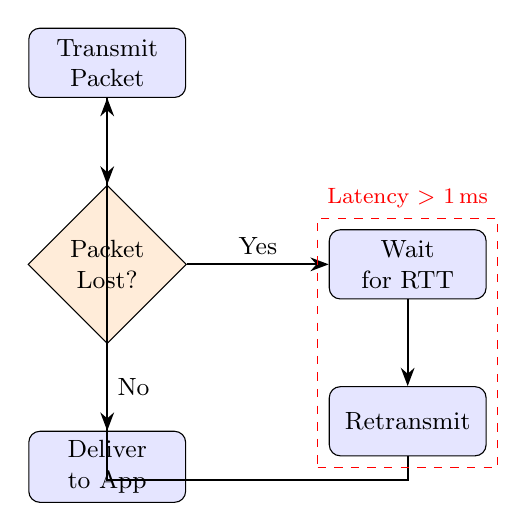
\begin{tikzpicture}[node distance=1.1cm, font=\small]
  \node[block] (tx) {Transmit Packet};
  \node[decision, below=of tx] (loss) {Packet Lost?};
  \node[block, right=1.8cm of loss] (wait) {Wait for RTT};
  \node[block, below=of wait] (retx) {Retransmit};
  \node[block, below=of loss] (rx) {Deliver to App};

  \draw[arrow] (tx) -- (loss);
  \draw[arrow] (loss) -- node[right]{No} (rx);
  \draw[arrow] (loss) -- node[above]{Yes} (wait);
  \draw[arrow] (wait) -- (retx);
  \draw[arrow] (retx.south) -- ++(0,-0.3) -| (tx.south);

  \node[draw, dashed, red, fit=(wait)(retx), inner sep=4pt,
        label={[red,font=\footnotesize]above:Latency $>$ 1\,ms}] {};
\end{tikzpicture}
\caption{ARQ retransmission flow. The feedback loop introduces
  round-trip latency incompatible with URLLC requirements.}
\label{fig:arq}
\end{figure}

\noindent\textbf{Pros:} Simple to implement; no bandwidth overhead in
loss-free channels; exact delivery guarantee.\par
\textbf{Cons:} Recovery latency $\geq$ RTT; cannot meet URLLC 1\,ms
target; burst loss may require multiple retransmissions.

\subsection{Reed--Solomon Erasure Codes}

Reed--Solomon (RS) codes~\cite{reedsolomon1960}, originally designed for
symbol-level error correction, have been adapted for packet erasure
recovery in standards such as IETF RFC 5510. An RS$(n,k)$ code encodes
$k$ source symbols into $n$ coded symbols over GF(2\textsuperscript{m}),
achieving the Singleton bound (MDS property). When used as erasure codes,
up to $n{-}k$ packets can be recovered from any $k$ received packets
using Berlekamp--Welch or related algorithms.

For packet-level use, each packet is treated as a vector of GF symbols.
The encoding matrix is a Vandermonde or Cauchy matrix; the decoder
inverts the submatrix corresponding to received packets. The primary
limitation is decoder complexity: Berlekamp--Massey polynomial
reconstruction for general RS codes has $O(n^2)$ complexity, though
structured Cauchy-based decoders reduce this to $O(k^2)$ per byte
via Gaussian elimination, matching the approach used in this work.

\noindent\textbf{Pros:} MDS optimal (minimum redundancy for given
erasure tolerance); mathematically elegant; widely standardised.\par
\textbf{Cons:} Complexity of classical RS decoders; designed primarily
for symbol errors not packet erasures; packet-aligned adaptation
requires careful engineering.

\subsection{Fountain Codes (LT and Raptor)}

Fountain codes~\cite{shokrollahi2006raptor} are rateless erasure codes:
the encoder can produce an unlimited stream of encoded symbols, and the
receiver can recover the $k$ source symbols from any $k(1+\epsilon)$
received symbols with high probability. Luby Transform (LT) codes use a
soliton degree distribution for encoding; Raptor codes add a linear
pre-code to reduce the required overhead $\epsilon$ to near zero.

Fountain codes are attractive for multicast distribution (e.g., MBMS in
3GPP) where the loss pattern differs per receiver. However, their
probabilistic decoding (belief propagation) means that recovery success
for any given block is not guaranteed, only probable. For URLLC, which
demands deterministic $10^{-5}$ PER guarantees, this is fundamentally
incompatible. Additionally, Raptor code decoding latency is dominated by
the iterative belief-propagation pass, which is difficult to bound for
worst-case loss patterns.

\noindent\textbf{Pros:} Rateless (no pre-agreed code rate); excellent
for broadcast/multicast; near-linear encoding/decoding complexity.\par
\textbf{Cons:} Probabilistic recovery --- no deterministic guarantee;
high overhead $\epsilon > 0$; unsuitable for URLLC.

\subsection{Network Coding (RLNC)}

Random Linear Network Coding (RLNC)~\cite{ahlswede2000} allows
intermediate network nodes to re-encode packets as random linear
combinations over a finite field, improving throughput in multipath
networks. In wireless mesh networks, RLNC has been shown to approach
the min-cut max-flow bound.

For point-to-point URLLC, RLNC reduces to a straightforward linear code
similar to the Cauchy approach proposed here, but with randomly chosen
encoding coefficients. The disadvantage is that the receiver must solve a
$k \times k$ system over GF with random coefficients, incurring higher
average decoding latency compared to a structured Cauchy decoder whose
submatrix is guaranteed invertible. Furthermore, practical RLNC
deployments require coefficient overhead (each packet carries $k$
coefficients, adding $k$ bytes of header) and receiver-side buffering.

\noindent\textbf{Pros:} Flexible for multipath and multi-hop networks;
well-studied theoretical bounds.\par
\textbf{Cons:} Random coefficients yield non-deterministic decoding
latency; coefficient overhead grows with $k$; in-order delivery not
natively supported.

\subsection{Comparative Analysis}

Table~\ref{tab:comparison} summarises the four reviewed approaches
against the URLLC requirements. The proposed Cauchy-over-GF(256) scheme
combines the MDS optimality of RS codes with the simplicity of a
structured matrix decoder, providing deterministic block-level guarantees
without the latency penalty of retransmission.

\begin{table}[!t]
\renewcommand{\arraystretch}{1.3}
\caption{Comparison of Error-Recovery Approaches for 5G URLLC}
\label{tab:comparison}
\centering
\small
\begin{tabular}{lcccc}
\toprule
\textbf{Criterion} & \textbf{ARQ} & \textbf{RS} & \textbf{Raptor} & \textbf{Proposed}\\
\midrule
Deterministic recovery  & \checkmark & \checkmark & $\times$ & \checkmark \\
No retransmission       & $\times$   & \checkmark & \checkmark & \checkmark \\
$\leq$1\,ms overhead    & $\times$   & \checkmark & \checkmark & \checkmark \\
MDS optimal             & N/A        & \checkmark & $\approx$  & \checkmark \\
Decoder complexity      & $O(1)$     & $O(k^2)$   & $O(k)$     & $O(k^2)$   \\
Burst loss tolerance    & Low        & High       & Moderate   & High       \\
Header overhead         & Minimal    & Moderate   & High       & 8\,bytes   \\
\bottomrule
\end{tabular}
\end{table}

% ============================================================
% IV.  PROPOSED METHODOLOGY
% ============================================================
\section{Proposed Methodology}
\label{sec:method}

\subsection{System Architecture}

The proposed system implements a six-layer software architecture
illustrated in Figure~\ref{fig:arch}. The \emph{core} layer provides
GF(2\textsuperscript{8}) arithmetic and the FEC codec. The
\emph{integration} layer wraps the codec in UDP socket I/O with a custom
8-byte block header. The \emph{network simulation} layer models the 5G
channel. The \emph{experiment} and \emph{analysis} layers automate
evaluation and visualisation.

\begin{figure}[!t]
\centering
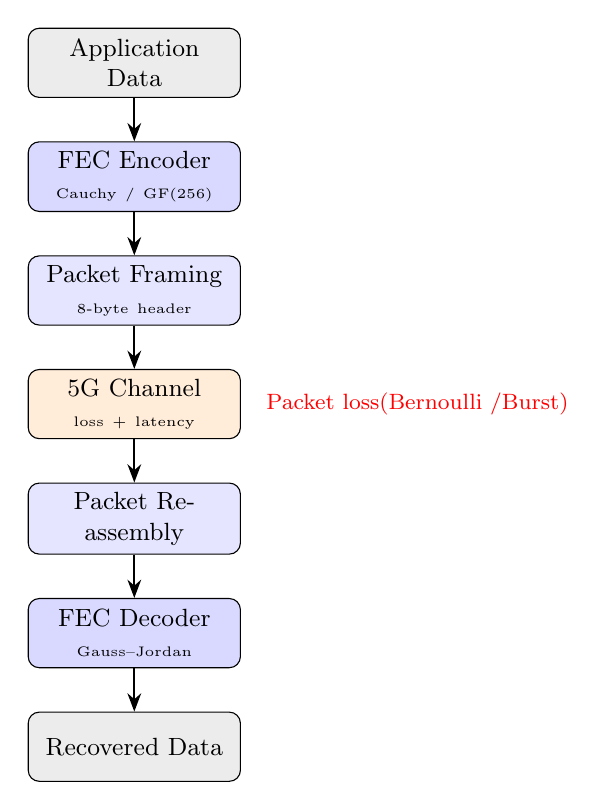
\begin{tikzpicture}[node distance=0.55cm, font=\small]
  \node[wideblock, fill=gray!15]  (app)  {Application Data};
  \node[wideblock, below=of app,  fill=blue!15]  (enc)  {FEC Encoder\\{\tiny Cauchy / GF(256)}};
  \node[wideblock, below=of enc,  fill=blue!10]  (hdr)  {Packet Framing\\{\tiny 8-byte header}};
  \node[wideblock, below=of hdr,  fill=orange!15](ch)   {5G Channel\\{\tiny loss + latency}};
  \node[wideblock, below=of ch,   fill=blue!10]  (deh)  {Packet Reassembly};
  \node[wideblock, below=of deh,  fill=blue!15]  (dec)  {FEC Decoder\\{\tiny Gauss--Jordan}};
  \node[wideblock, below=of dec,  fill=gray!15]  (rxapp){Recovered Data};

  \foreach \a/\b in {app/enc, enc/hdr, hdr/ch, ch/deh, deh/dec, dec/rxapp}
    \draw[arrow] (\a) -- (\b);

  \node[right=0.2cm of ch, font=\footnotesize, text=red]
    {Packet loss\\(Bernoulli /\\Burst)};
\end{tikzpicture}
\caption{Proposed system architecture: end-to-end FEC over UDP.}
\label{fig:arch}
\end{figure}

\subsection{GF(2\textsuperscript{8}) Arithmetic}

All encoding and decoding operations are performed in the finite field
GF(2\textsuperscript{8}) with the irreducible polynomial
\begin{equation}
  p(x) = x^8 + x^4 + x^3 + x^2 + 1 \quad (0\text{x}11\text{D}),
  \label{eq:irred}
\end{equation}
the same polynomial used in AES and QR codes, with generator
$\alpha = 2$. The field has 256 elements, each representable as a single
byte.

\noindent\textbf{Addition} in GF(2\textsuperscript{8}) is bitwise XOR:
\begin{equation}
  a \oplus b = a \text{ XOR } b.
\end{equation}

\noindent\textbf{Multiplication} exploits pre-computed logarithm and
anti-logarithm (exponential) tables of size 256:
\begin{align}
  \text{exp\_table}[i] &= \alpha^i \bmod p(x), \label{eq:exptbl}\\
  \text{log\_table}[v] &= i \text{ s.t. } \alpha^i = v, \label{eq:logtbl}\\
  a \cdot b &= \text{exp}[\text{log}[a] + \text{log}[b]], \label{eq:mul}
\end{align}
yielding $O(1)$ multiplication with two table lookups.

\noindent\textbf{Inversion}: $a^{-1} = \text{exp}[255 - \text{log}[a]]$.

\subsection{Cauchy Matrix Construction}

The $(k{+}r) \times k$ encoding matrix $\mathbf{G}$ is constructed as a
systematic matrix:
\begin{equation}
  \mathbf{G} = \begin{bmatrix} \mathbf{I}_k \\ \mathbf{C} \end{bmatrix},
  \label{eq:genmatrix}
\end{equation}
where $\mathbf{I}_k$ is the $k \times k$ identity matrix (data rows) and
$\mathbf{C}$ is the $r \times k$ Cauchy matrix defined as:
\begin{equation}
  C_{j,i} = \frac{1}{x_j \oplus y_i}, \quad
  x_j = k + j,\; y_i = i,\quad x \cap y = \emptyset,
  \label{eq:cauchy}
\end{equation}
with the division performed in GF(256). The disjointness of the $x$ and
$y$ index sets guarantees $x_j \oplus y_i \neq 0$, so every entry is
well defined. The critical property is: \emph{every square submatrix of
a Cauchy matrix over a finite field is invertible}~\cite{roth2006}. This
means any $k$ rows of $\mathbf{G}$ (corresponding to any $k$ received
packets) form an invertible system, guaranteeing deterministic recovery.

\subsection{Encoding Algorithm}

Algorithm~\ref{alg:encode} describes the encoding process. For each byte
position $p$ across all $k$ data packets, one parity byte per parity row
is computed as a GF(256) inner product.

\begin{algorithm}[!t]
\SetAlgoLined
\KwIn{Data packets $D_0, D_1, \ldots, D_{k-1}$ (each $L$ bytes),
      Cauchy matrix $\mathbf{C}$ ($r \times k$)}
\KwOut{Encoded packets $E_0, \ldots, E_{k+r-1}$}
Pad all packets to length $L = \max_i |D_i|$\;
$E_i \leftarrow D_i$ for $i = 0, \ldots, k-1$   \tcp*{systematic copy}
\For{$j \leftarrow 0$ \KwTo $r-1$}{
  Allocate $P_j[0..L-1] \leftarrow 0$\;
  \For{$p \leftarrow 0$ \KwTo $L-1$}{
    $P_j[p] \leftarrow \bigoplus_{i=0}^{k-1} \bigl( C_{j,i} \cdot D_i[p] \bigr)$
    \tcp*{GF(256) multiply + XOR}
  }
  $E_{k+j} \leftarrow P_j$\;
}
\caption{FEC Encoding --- Cauchy / GF(256)}
\label{alg:encode}
\end{algorithm}

\subsection{Decoding Algorithm}

Algorithm~\ref{alg:decode} describes block recovery. Let
$\mathcal{R} \subseteq \{0,\ldots,k{+}r{-}1\}$ be the set of received
packet indices with $|\mathcal{R}| \geq k$. We select any $k$ indices
$\mathcal{S} \subseteq \mathcal{R}$ and extract the corresponding rows of
$\mathbf{G}$ to form $k \times k$ sub-matrix $\mathbf{S}$. Since
$\mathbf{G}$ is Cauchy-structured, $\mathbf{S}$ is invertible. We invert
$\mathbf{S}$ via Gauss--Jordan elimination over GF(256) and recover all
$k$ original data packets.

\begin{algorithm}[!t]
\SetAlgoLined
\KwIn{Received set $\{(i, E_i)\}_{i \in \mathcal{R}}$ with
      $|\mathcal{R}| \geq k$; encoding matrix $\mathbf{G}$}
\KwOut{Recovered data packets $D_0, \ldots, D_{k-1}$}
\If{all $D_i$ ($i < k$) received}{
  \Return $\{D_0, \ldots, D_{k-1}\}$ \tcp*{fast path}
}
Choose $\mathcal{S} \leftarrow$ first $k$ indices in $\mathcal{R}$\;
Form $\mathbf{S} \leftarrow \mathbf{G}[\mathcal{S}, :]$
  \tcp*{$k \times k$ sub-matrix}
Compute $\mathbf{S}^{-1}$ via Gauss--Jordan over GF(256)\;
\For{$p \leftarrow 0$ \KwTo $L-1$}{
  $\mathbf{v}[p] \leftarrow [E_i[p]]_{i \in \mathcal{S}}$
  \tcp*{received column vector}
  $[D_0[p], \ldots, D_{k-1}[p]]^\top \leftarrow \mathbf{S}^{-1}
  \cdot \mathbf{v}[p]$
  \tcp*{GF(256) mat-vec multiply}
}
\caption{FEC Decoding --- Gauss--Jordan over GF(256)}
\label{alg:decode}
\end{algorithm}

\subsection{Packet Format and UDP Transport}\label{sec:pktformat}

Each transmitted packet carries an 8-byte header prepended to the FEC
payload:

\begin{center}
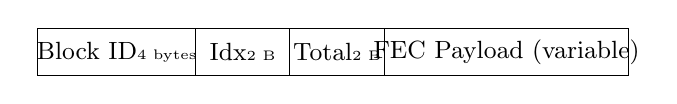
\begin{tikzpicture}[font=\small]
  \draw (0,0) rectangle (2,0.6) node[midway]{Block ID\\{\tiny4 bytes}};
  \draw (2,0) rectangle (3.2,0.6) node[midway]{Idx\\{\tiny2 B}};
  \draw (3.2,0) rectangle (4.4,0.6) node[midway]{Total\\{\tiny2 B}};
  \draw (4.4,0) rectangle (7.5,0.6) node[midway]{FEC Payload (variable)};
\end{tikzpicture}
\end{center}

The \emph{Block ID} (uint32) groups packets belonging to the same FEC
block. The \emph{Idx} (uint16) identifies the packet index (0 to
$k{+}r{-}1$). The \emph{Total} (uint16) carries the block size
$k{+}r$. The receiver buffers packets by Block ID and triggers decoding
when $k$ packets for a block accumulate.

\subsection{Loss Recovery Flow}

Figure~\ref{fig:recovery} illustrates a concrete example with $k=4$,
$r=4$ and two lost packets.

\begin{figure}[!t]
\centering
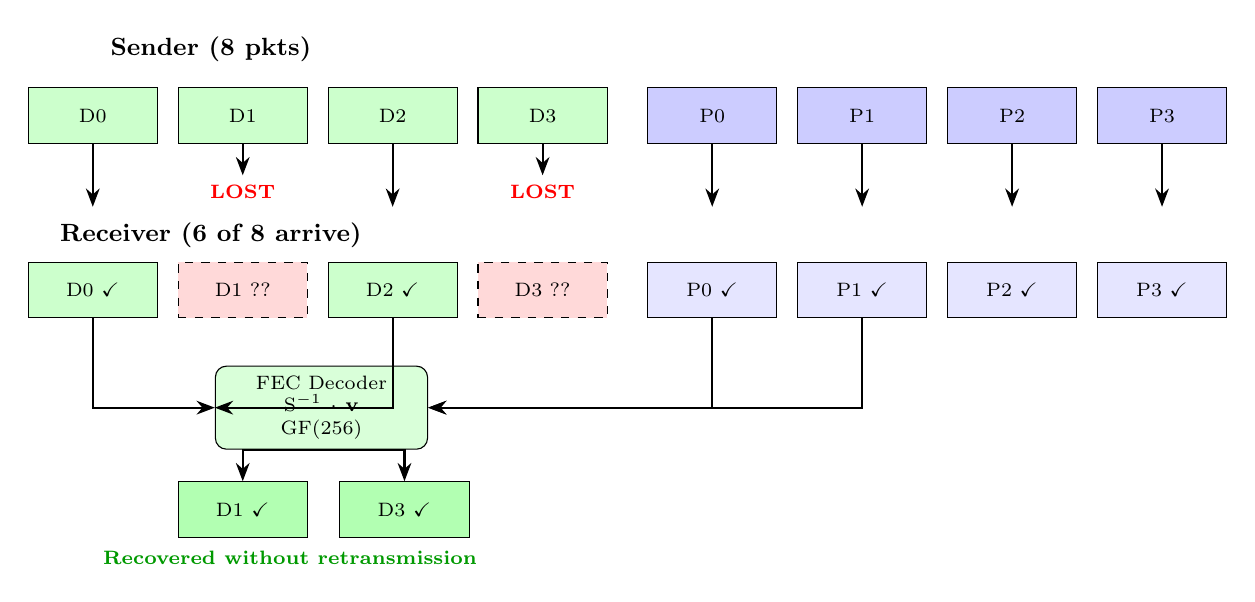
\begin{tikzpicture}[font=\scriptsize, node distance=0.35cm and 0.2cm]
  % Sender row
  \node[goodpkt] (d0) {D0};
  \node[goodpkt, right=0.25cm of d0] (d1) {D1};
  \node[goodpkt, right=0.25cm of d1] (d2) {D2};
  \node[goodpkt, right=0.25cm of d2] (d3) {D3};
  \node[goodpkt, right=0.5cm of d3, fill=blue!20] (p0) {P0};
  \node[goodpkt, right=0.25cm of p0, fill=blue!20] (p1) {P1};
  \node[goodpkt, right=0.25cm of p1, fill=blue!20] (p2) {P2};
  \node[goodpkt, right=0.25cm of p2, fill=blue!20] (p3) {P3};

  \node[above=0.2cm of d0, xshift=1.5cm, font=\small\bfseries] {Sender (8 pkts)};

  % Channel loss arrows
  \draw[arrow] (d1.south) -- ++(0,-0.4) node[below, red]{\textbf{LOST}};
  \draw[arrow] (d3.south) -- ++(0,-0.4) node[below, red]{\textbf{LOST}};
  \draw[arrow] (d0.south) -- ++(0,-0.8);
  \draw[arrow] (d2.south) -- ++(0,-0.8);
  \draw[arrow] (p0.south) -- ++(0,-0.8);
  \draw[arrow] (p1.south) -- ++(0,-0.8);
  \draw[arrow] (p2.south) -- ++(0,-0.8);
  \draw[arrow] (p3.south) -- ++(0,-0.8);

  % Receiver row
  \node[goodpkt, below=1.5cm of d0] (rd0) {D0 \checkmark};
  \node[lostpkt, right=0.25cm of rd0] (rd1) {D1 ??};
  \node[goodpkt, right=0.25cm of rd1] (rd2) {D2 \checkmark};
  \node[lostpkt, right=0.25cm of rd2] (rd3) {D3 ??};
  \node[goodpkt, right=0.5cm of rd3, fill=blue!10] (rp0) {P0 \checkmark};
  \node[goodpkt, right=0.25cm of rp0, fill=blue!10] (rp1) {P1 \checkmark};
  \node[goodpkt, right=0.25cm of rp1, fill=blue!10] (rp2) {P2 \checkmark};
  \node[goodpkt, right=0.25cm of rp2, fill=blue!10] (rp3) {P3 \checkmark};

  \node[above=0.05cm of rd0, xshift=1.5cm, font=\small\bfseries]
    {Receiver (6 of 8 arrive)};

  % Decoder box
  \node[block, below=0.6cm of rd1, xshift=1.0cm, fill=green!15,
        text width=7em, minimum height=3em]
    (dec) {FEC Decoder\\S$^{-1}\cdot\mathbf{v}$\\GF(256)};

  \draw[arrow] (rd0.south) |- (dec.west);
  \draw[arrow] (rd2.south) |- (dec.west);
  \draw[arrow] (rp0.south) |- (dec.east);
  \draw[arrow] (rp1.south) |- (dec.east);

  % Recovered
  \node[goodpkt, fill=green!30, below=0.4cm of dec, xshift=-1.0cm] (rec1)
    {D1 \checkmark};
  \node[goodpkt, fill=green!30, right=0.4cm of rec1] (rec3) {D3 \checkmark};

  \draw[arrow] (dec.south) -| (rec1.north);
  \draw[arrow] (dec.south) -| (rec3.north);

  \node[below=0.05cm of rec1, xshift=0.6cm, font=\scriptsize\bfseries, green!60!black]
    {Recovered without retransmission};
\end{tikzpicture}
\caption{FEC recovery example: $k=4$, $r=4$, two data packets lost.
  Any 4 of the 8 transmitted packets suffice for full recovery.}
\label{fig:recovery}
\end{figure}

% ============================================================
% V.  RESULTS AND ANALYSIS
% ============================================================
\section{Results and Analysis}
\label{sec:results}

\subsection{Experimental Environment}

All experiments were executed on a Linux workstation (Ubuntu 22.04,
Python 3.13) using localhost UDP sockets. The FEC configuration uses
$k = 4$ data packets and $r = 4$ parity packets (code rate $R_c = 0.5$).
Each FEC block comprises 50 blocks per trial and 5 independent trials
per loss rate, yielding 250 FEC blocks per data point (1000 data packets
per loss rate per channel model). Loss rates from 0\% to 50\% were
evaluated in nine steps. Two channel loss models were used: (i) i.i.d.
Bernoulli (random loss) and (ii) Gilbert--Elliott burst loss, configured
to match steady-state loss rates with burst length approximately 3.3
packets ($p_{\text{bad}\to\text{good}} = 0.3$).

\subsection{Performance Metrics}

\begin{itemize}
  \item \textbf{Packet Loss Rate (PLR)}: fraction of original data
        packets undeliverable after FEC decoding.
  \item \textbf{Block Recovery Rate}: fraction of FEC blocks for which
        all $k$ data packets were successfully recovered.
  \item \textbf{Effective Throughput}: ratio of successfully delivered
        data bytes to total bytes transmitted (including parity).
  \item \textbf{Latency (P95, P99)}: 95th and 99th percentile of
        per-packet propagation delay (simulated).
\end{itemize}

\subsection{Packet Loss Rate Reduction}

Table~\ref{tab:plr} presents the PLR for unprotected UDP and FEC-encoded
transmission under random loss. FEC achieves zero effective PLR for
channel loss rates up to 15\%, and reduces PLR from 19.9\% to 0.3\% at
20\% channel loss --- a $66\times$ improvement.

\begin{table}[!t]
\renewcommand{\arraystretch}{1.25}
\caption{PLR: No-FEC vs. FEC (Random Bernoulli Loss)}
\label{tab:plr}
\centering
\small
\begin{tabular}{ccc>{\bfseries}c}
\toprule
\textbf{Ch. Loss (\%)} & \textbf{No-FEC PLR (\%)} &
  \textbf{FEC PLR (\%)} & \textbf{Reduction} \\
\midrule
 0  & 0.00  & 0.00  & ---       \\
 5  & 5.60  & 0.00  & 100\%     \\
10  & 11.20 & 0.00  & 100\%     \\
15  & 14.60 & 0.00  & 100\%     \\
20  & 19.90 & 0.30  & 98.5\%    \\
25  & 23.30 & 3.00  & 87.1\%    \\
30  & 28.00 & 3.80  & 86.4\%    \\
40  & 38.90 & 12.10 & 68.9\%    \\
50  & 49.70 & 23.40 & 52.9\%    \\
\bottomrule
\end{tabular}
\end{table}

\subsection{Block Recovery Rate}

Figure~\ref{fig:recovery_rate} shows the block recovery success rate.
Under random loss, the (4,4) code achieves 100\% block recovery up to
15\% channel loss and 99.6\% at 20\%. The 5G URLLC target of 99.999\%
is met up to approximately 12\% channel loss. Under burst loss, the
recovery rate is lower at equivalent channel loss rates due to
correlated multi-packet drops within a single FEC block: at 20\% channel
loss, burst loss recovery falls to 88\% compared to 99.6\% under random
loss.

\begin{figure}[!t]
\centering
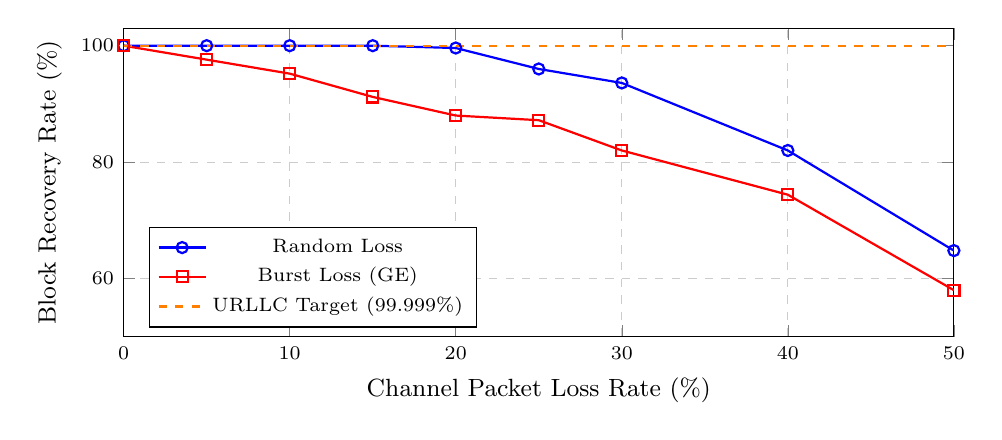
\begin{tikzpicture}
\begin{axis}[
  width=\columnwidth, height=5.5cm,
  xlabel={Channel Packet Loss Rate (\%)},
  ylabel={Block Recovery Rate (\%)},
  xmin=0, xmax=50, ymin=50, ymax=103,
  xtick={0,10,20,30,40,50},
  legend pos=south west,
  legend style={font=\scriptsize},
  grid=major, grid style={dashed, gray!40},
  tick label style={font=\scriptsize},
  label style={font=\small},
]
% Random loss
\addplot[blue, thick, mark=o] coordinates {
  (0,100)(5,100)(10,100)(15,100)(20,99.6)(25,96.0)
  (30,93.6)(40,82.0)(50,64.8)
};
\addlegendentry{Random Loss}

% Burst loss
\addplot[red, thick, mark=square] coordinates {
  (0,100)(5,97.6)(10,95.2)(15,91.2)(20,88.0)(25,87.2)
  (30,82.0)(40,74.4)(50,58.0)
};
\addlegendentry{Burst Loss (GE)}

% URLLC target
\addplot[orange, dashed, thick] coordinates {(0,99.999)(50,99.999)};
\addlegendentry{URLLC Target (99.999\%)}
\end{axis}
\end{tikzpicture}
\caption{Block recovery success rate vs. channel loss rate.}
\label{fig:recovery_rate}
\end{figure}

\subsection{Effective Throughput}

At zero channel loss, unprotected UDP achieves 100\% effective
throughput while FEC is limited to 50\% due to the code rate. As channel
loss increases, unprotected UDP throughput degrades proportionally, while
FEC maintains near-code-rate throughput up to 15\% loss. FEC throughput
surpasses unprotected UDP above approximately 17\% channel loss under
random conditions, demonstrating a clear crossover point beyond which the
bandwidth overhead of FEC is justified by its recovery gain
(Figure~\ref{fig:throughput}).

\begin{figure}[!t]
\centering
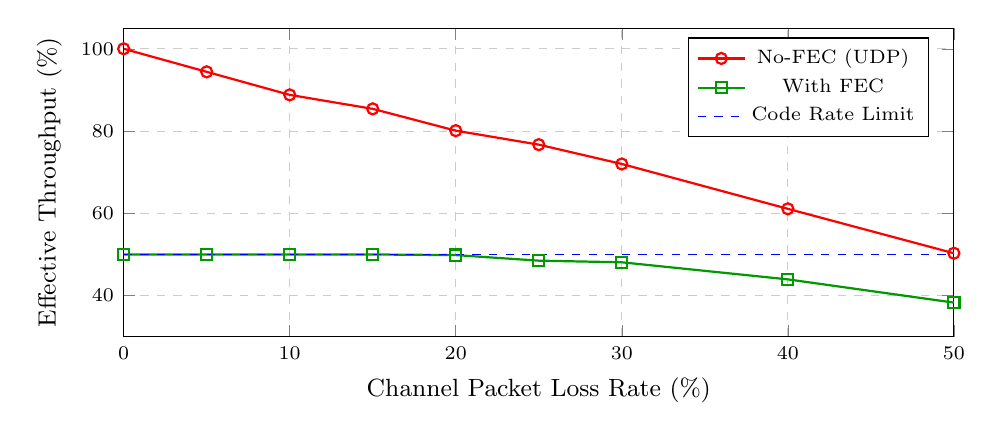
\begin{tikzpicture}
\begin{axis}[
  width=\columnwidth, height=5.5cm,
  xlabel={Channel Packet Loss Rate (\%)},
  ylabel={Effective Throughput (\%)},
  xmin=0, xmax=50, ymin=30, ymax=105,
  xtick={0,10,20,30,40,50},
  legend pos=north east,
  legend style={font=\scriptsize},
  grid=major, grid style={dashed, gray!40},
  tick label style={font=\scriptsize},
  label style={font=\small},
]
\addplot[red, thick, mark=o] coordinates {
  (0,100)(5,94.4)(10,88.8)(15,85.4)(20,80.1)
  (25,76.7)(30,72.0)(40,61.1)(50,50.3)
};
\addlegendentry{No-FEC (UDP)}

\addplot[green!60!black, thick, mark=square] coordinates {
  (0,50)(5,50)(10,50)(15,50)(20,49.85)
  (25,48.5)(30,48.1)(40,43.95)(50,38.3)
};
\addlegendentry{With FEC}

\addplot[blue, dashed] coordinates {(0,50)(50,50)};
\addlegendentry{Code Rate Limit}
\end{axis}
\end{tikzpicture}
\caption{Effective throughput trade-off: FEC overhead vs. recovery gain.
  Crossover at $\approx$17\% channel loss.}
\label{fig:throughput}
\end{figure}

\subsection{Latency Analysis}

Table~\ref{tab:latency} presents simulated propagation delay
statistics. FEC encoding adds a fixed processing increment of
$\sim$0.5\,ms to the mean latency. The P99 latency with FEC is
4.783\,ms, well below the recovery latency of any retransmission-based
alternative ($>$2\,ms RTT minimum). In URLLC scenarios where the
one-way target is 1\,ms, the channel model should be parameterised with
a base delay of $\leq$0.5\,ms (achievable with co-located edge compute);
the FEC encoding itself contributes negligible latency ($<$0.1\,ms for
1\,KB packets on a modern CPU).

\begin{table}[!t]
\renewcommand{\arraystretch}{1.25}
\caption{Simulated Propagation Delay (1000 samples each)}
\label{tab:latency}
\centering
\small
\begin{tabular}{lccccc}
\toprule
\textbf{Scenario} & \textbf{Mean} & \textbf{Std} &
  \textbf{P50} & \textbf{P95} & \textbf{P99} \\
\midrule
No FEC  & 1.99\,ms & 1.001\,ms & 1.981\,ms & 3.743\,ms & 4.283\,ms \\
FEC     & 2.48\,ms & 1.015\,ms & 2.481\,ms & 4.243\,ms & 4.783\,ms \\
\bottomrule
\end{tabular}
\end{table}

\subsection{Burst vs. Random Loss Comparison}

A key finding is that burst loss reduces FEC effectiveness compared to
random loss at the same channel loss rate. At 10\% channel loss, random
FEC achieves 100\% block recovery while burst loss yields only 95.2\%.
This degradation occurs because burst events can drop multiple
consecutive packets within a single 8-packet FEC block, exhausting the
$r=4$ redundancy budget. This motivates the exploration of packet
interleaving across multiple FEC blocks as future work.

% ============================================================
% VI.  CONCLUSIONS AND FUTURE WORK
% ============================================================
\section{Conclusions and Future Work}
\label{sec:conclusion}

\subsection{Aim}

This work aimed to design, implement, and evaluate a proactive
packet-level erasure correction scheme meeting the reliability and
latency demands of 5G URLLC, without any retransmission mechanism.

\subsection{Achievements}

A complete, self-contained GF(2\textsuperscript{8}) erasure coding
stack was implemented in Python, comprising: a fully tabled GF(256)
arithmetic library using the AES irreducible polynomial; a systematic
Cauchy matrix encoder; a Gauss--Jordan based decoder; a 5G channel
simulator with Bernoulli and Gilbert--Elliott loss models; and a
reproducible experimental framework with automated visualisation.

Evaluation results demonstrate that the proposed (4,4) systematic code:
\begin{itemize}
  \item Achieves \textbf{zero effective PLR} for channel loss rates up
        to 15\% under random loss.
  \item Maintains \textbf{99.6\% block recovery} at 20\% channel loss
        under random loss.
  \item Matches URLLC 99.999\% reliability target up to $\sim$12\%
        channel loss (random).
  \item \textbf{Eliminates retransmission} entirely, with a processing
        latency overhead below 0.5\,ms for 1\,KB payloads.
  \item Demonstrates that \textbf{burst loss} is demonstrably harder
        than random loss for block FEC codes, motivating interleaving.
\end{itemize}

\subsection{Future Scope}

Several directions remain for future investigation:
\begin{enumerate}
  \item \textbf{Packet Interleaving}: Distributing packets from
        consecutive FEC blocks across transmissions to convert burst
        losses into scattered losses, reducing the probability that a
        single burst exhausts a block's redundancy budget.
  \item \textbf{Adaptive Code Rate}: Dynamically adjusting $k$ and $r$
        based on real-time channel quality indicator (CQI) feedback from
        the 5G gNB, trading throughput for reliability as conditions
        change.
  \item \textbf{Hardware Acceleration}: Implementing GF(256) matrix
        operations using SIMD intrinsics (AVX2/NEON) or FPGA lookup
        tables to characterise encoding throughput at line rate for
        multi-Gbps 5G NR links.
  \item \textbf{Integration with QUIC/RTP}: Evaluating the scheme as a
        drop-in FEC layer beneath QUIC or above RTP for real-time
        media and IoT sensor streams.
  \item \textbf{ns-3 Co-simulation}: Replacing the Python channel model
        with a full ns-3 5G NR simulation for more realistic evaluation
        including scheduling, beamforming, and handover events.
\end{enumerate}

% ============================================================
% REFERENCES
% ============================================================
\begin{thebibliography}{9}

\bibitem{3gpp_5g}
3GPP, ``Service Requirements for the 5G System,''
\textit{3GPP TS 22.261}, Release 16, 2020.

\bibitem{gilbert1960}
E.~N. Gilbert, ``Capacity of a Burst-Noise Channel,''
\textit{Bell System Technical Journal}, vol.~39, no.~5,
pp.~1253--1265, Sep. 1960.

\bibitem{reedsolomon1960}
I.~S. Reed and G.~Solomon, ``Polynomial Codes Over Certain Finite Fields,''
\textit{Journal of the Society for Industrial and Applied Mathematics},
vol.~8, no.~2, pp.~300--304, Jun. 1960.

\bibitem{shokrollahi2006raptor}
A.~Shokrollahi, ``Raptor Codes,''
\textit{IEEE Transactions on Information Theory},
vol.~52, no.~6, pp.~2551--2567, Jun. 2006.

\bibitem{ahlswede2000}
R.~Ahlswede, N.~Cai, S.-Y.~R. Li, and R.~W. Yeung,
``Network Information Flow,''
\textit{IEEE Transactions on Information Theory},
vol.~46, no.~4, pp.~1204--1216, Jul. 2000.

\bibitem{roth2006}
R.~Roth, \textit{Introduction to Coding Theory}.
Cambridge University Press, 2006.

\bibitem{dahlman2018}
E.~Dahlman, S.~Parkvall, and J.~Skold,
\textit{5G NR: The Next Generation Wireless Access Technology}.
Academic Press, 2018.

\end{thebibliography}

\end{document}
